%Custom Functions
\newcommand{\CompanyName}{TT} % update later

\documentclass[conference]{IEEEtran}
\IEEEoverridecommandlockouts
% The preceding line is only needed to identify funding in the first footnote. If that is unneeded, please comment it out.
%\usepackage{cite}
\usepackage{amsmath,amssymb,amsfonts}
\usepackage{algorithmic}
\usepackage{graphicx}
\usepackage{textcomp}
\usepackage{xcolor}

\usepackage{pdflscape}

\usepackage[utf8]{inputenc}
\usepackage{fancyhdr}
\usepackage{lastpage}

% Please add the following required packages to your document preamble:
\usepackage{multirow}
\usepackage[numbers]{natbib}

\usepackage{listings}
\usepackage{hyperref}
\usepackage{amsmath}

\hypersetup{
    colorlinks=true,
    linkcolor=black,
    filecolor=magenta,      
	urlcolor=cyan
}

\usepackage{listings}
\usepackage{color}

\definecolor{dkgreen}{rgb}{0,0.6,0}
\definecolor{gray}{rgb}{0.5,0.5,0.5}
\definecolor{mauve}{rgb}{0.58,0,0.82}

\lstset{frame=single,
  language=C++,
  showstringspaces=false,
  columns=flexible,
  basicstyle={\small\ttfamily},
  numbers = none,
  numberstyle=\tiny\color{gray},
  keywordstyle=\color{blue},
  commentstyle=\color{dkgreen},
  stringstyle=\color{mauve},
  breaklines=true,
  breakatwhitespace=true,
  tabsize=2
}

\def\BibTeX{{\rm B\kern-.05em{\sc i\kern-.025em b}\kern-.08em
T\kern-.1667em\lower.7ex\hbox{E}\kern-.125emX}}

\fancypagestyle{fancylandscape}{
\fancyhf{} %Clears the header/footer
\fancyfoot{% Footer
\makebox[\textwidth][r]{% Right
  \rlap{\hspace{.75cm}% Push out of margin by \footskip
    \smash{% Remove vertical height
      \raisebox{4.87in}{% Raise vertically
        \rotatebox{90}{Page \thepage\ of \pageref{LastPage}}}}}}}% Rotate counter-clockwise
\renewcommand{\headrulewidth}{0pt}% No header rule
\renewcommand{\footrulewidth}{0pt}% No footer rule
}

\pagestyle{fancyplain}
\fancyhf{}
\fancyfoot[c]{Page \thepage\ of \pageref{LastPage}}
\renewcommand{\headrulewidth}{0pt}

\begin{document}

	\title{VisualPro - Research Proposal}

	\author{\IEEEauthorblockN{1\textsuperscript{st} Given Edward Patch}
	\IEEEauthorblockA{\textit{Software Engineer Student (of BSc Year 3)} \\
    \textit{Independent Project}\\
    \textit{University of Wales Trinity St. Davids (of Mike Dacey)}\\
    Swansea, Wales \\
    Student ID: 1801492}}

     \maketitle
    
    \thispagestyle{plain}
    \pagestyle{plain}
    
    \tableofcontents
	  \vspace{.5cm}
    %\newpage
	
    \begin{abstract}
      This document provides the proposal of the Independent Project. After doing in-depth research and planning, the working title for this project is VisualPro.

      Hypothesis: If visual scripting can write structure and logic of any desired language the user wishes, will this:-
        \begin{itemize}
          \item A: produce a more productive and better work environment.
          \item B: help newcomers code in any language without knowing different syntax per language.
        \end{itemize}
       
    \end{abstract}

    \begin{IEEEkeywords}
        Visual Programming, Proposal, Research.
    \end{IEEEkeywords}
  
    \section{Introduction}
      VisualPro aims to be a lightweight visual programming pad, which includes the following features:-
      \begin{itemize}
        \item Program in any language with ease.
        \item Enables users to write code in minutes.
        \item A simple Graphical User Interface (GUI) that changes the way Visual Scripting already works.
      \end{itemize}
  
      The prototypes will demonstrate C/C++ libraries working together with a different language, which plays a massive part to archive this task.

      \subsection{Potential growth to VisualPro}
      The dynamics of the custom languages allow new scripting languages. Consequently, it implies but is not limited to, Notebook and Stylus companies benefiting from this product. Take a look at (reference page) for more information on this topic.

      \subsection{Sections}
      The VisualPro Proposal document includes a Literature Review, Aims and Objective, Project Design, Resources and Planning and Reference List.

      The Literature Review section contains segments of academic books and journals related to the project proposal. Within the extensive research, hand-picked articles and journals to show what technologies are required to make the idea plausible, narrowing down the project's association towards the author's study area.
      
      After the Literature Review section, the Aims and Objectives section will give the reader an idea of how the final product will impact society and its user base.
      
      The third section, Project Design, describes the outline of the project process, data collection, risks and limitations and ethical issues. These are essential points that decide if the project breaks any laws or pushes too many boundaries in today's society.
      
      The Resources and Planning section include two sub-sections; Resources Required and Planning Chart. Resources Required sub-section involves Physical Resources \textit{(if any hardware and equipment are required)}, Human Resources \textit{(if any staff are required)} and Other Resources \textit{(if any software or other categories not been mentioned are required)}. The planning Chart sub-section displays the tasks and time frame within a Gantt Chart, constructed by Microsoft Project~\cite{microsoft_compare_nodate}.
    \section{Literature Review}
    \label{sec:literatureReview}
      \subsection{Productivity}
      \subsection{Visual Scripting}
      \subsection{Markup Languages}
      \label{subsec:lr-markupLanguages}
        \textbf{What is a Markup Language?}
          After studying Markup Languages: Theory and Practice Scope Statement~\cite{noauthor_markup_1999} Journal Article, page 46 by and Learning XML (Extensible Markup Language), Erik T. Ray's~\cite{ray_learning_nodate} Book, Chapter 2 (Markup and Core Concepts), page 49, a few points were selected to explain what is a markup language. A markup language is essentially a script, which consists of tags and attributes. 

          From Erik T. Ray's~\cite{ray_learning_nodate} Book, "Just as skeletons give us vertebrates shape and structure, markup does the same for text." This quote implies that markup languages offer structures, principally for designs, layouts and arrangement responsibilities. Due to the nature of Markup Languages with the ease of adding tags and attributes, Markup Languages will do the heavy lifting of setting available libraries and syntax for each language.

        \textbf{How will Extensible Markup Language (XML) support custom languages in this project?}

    \section{Aims and Objectives}
      \subsection{Aims}
        VisualPro software aims to increase existing software engineers, web developers, and other users in different professions. Productivity would increase and allow individuals to code in many languages without understanding different languages. The software aims to provide custom languages by a markup language with an easy-to-grasp script. Read section~\ref{sec:literatureReview} Literature Review, sub-section~\ref{subsec:lr-markupLanguages}, page~\pageref{subsec:lr-markupLanguages} to understand markup language.
      \subsection{Objectives}
        To achieve the aims mentioned in section~(a reference in aims and objectives), sub-section~(a reference in arms). In order to meet the aims during the production process of the project, the following objectives is a must. These objectives are as follows:-
        \begin{itemize}
          \item Project planning (section:~\ref{sec: resourcesPlanning} Resources and Planning, sub-section:~\ref{subsec:rp-planningChart} Planning Chart, page~\pageref{subsec:rp-planningChart}).
          \item Create prototypes (Existing \href{https://github.com/ShinkuKira21/VisualPro-FinalProject/tree/main/Experience}{programs}~\cite{patch_programming_2021} and \href{https://github.com/ShinkuKira21/VisualPro-FinalProject/tree/main/Libraries}{libraries}~\cite{patch_libraries_2021} to make this possible.).
          \item Create a frontend to work with existing libraries.
          \item Create a backend to communicate with the frontend and generate code based on values the user enters.
        \end{itemize}
      
    \section{Project Design}
      \subsection{Outline of Project Process}
        Outline of the project process:-
        \begin{itemize}
          \item Design and produce a frontend to dock the backend libraries.
          \item Convert existing libraries and programs to Dynamic-Link Library (DLL) archives that work with the frontend.
          \item Create a LanguageCompiler (similarly to \href{https://github.com/ShinkuKira21/VisualPro-FinalProject/tree/main/Experience}{Programming Planner}~\cite{patch_programming_2021}) but with custom languages (XML).
          \item Design and create an XML script that tells the backend of what languages are available. The script must be understandable by the user.
          \item Use C \_declspec(dllexport) to export entry points within the DLL libraries.
        \end{itemize}
        
      \subsection{Data Collection}
        Survey data will not ask for the personal details of the surveyed as it is not applicable data. When using the software, VisualPro, user data is not needed to operate this application. However, if the software is enhanced, author information may happen to be recorded in the future.

      \subsection{Risks and Limitations}
        
      \subsection{Ethical Issues}
    \section{Resources and Planning}
    \label{sec: resourcesPlanning}
      \subsection{Resources Required}
        \textbf{Physical Resources}

        \textbf{Human Resources}

        \textbf{Other Resources}

      \subsection{Planning Chart}
      \label{subsec:rp-planningChart}
        After planning the schedule to 400 hours to fit in the 28$^{\text{th}}$ of April 2022 deadline, the schedule finishes on the 07${\text{th}}$ of April 2022, giving leeway of 21 days. 

        Schedule of VisualPro:~\href{https://github.com/ShinkuKira21/VisualPro-FinalProject/blob/main/Project/VisualPro.mpp?raw=true}{Microsoft Project Schedule}~\cite{patch_visualpro_2021}.
        
        Evidence of~\href{https://github.com/ShinkuKira21/VisualPro-FinalProject/blob/main/Project/Plan.docx?raw=true}{Microsoft Project Schedule}~\cite{patch_visualpro_2021-1}.

      %SUBSECTION LANDSCAPE
      \begin{landscape}
        \thispagestyle{fancylandscape}
        \subsection{Mindmap - Ideas}
        This mindmap demonstrates the process and current experience, which helped get the idea for the final project.
        \begin{figure}[h]
          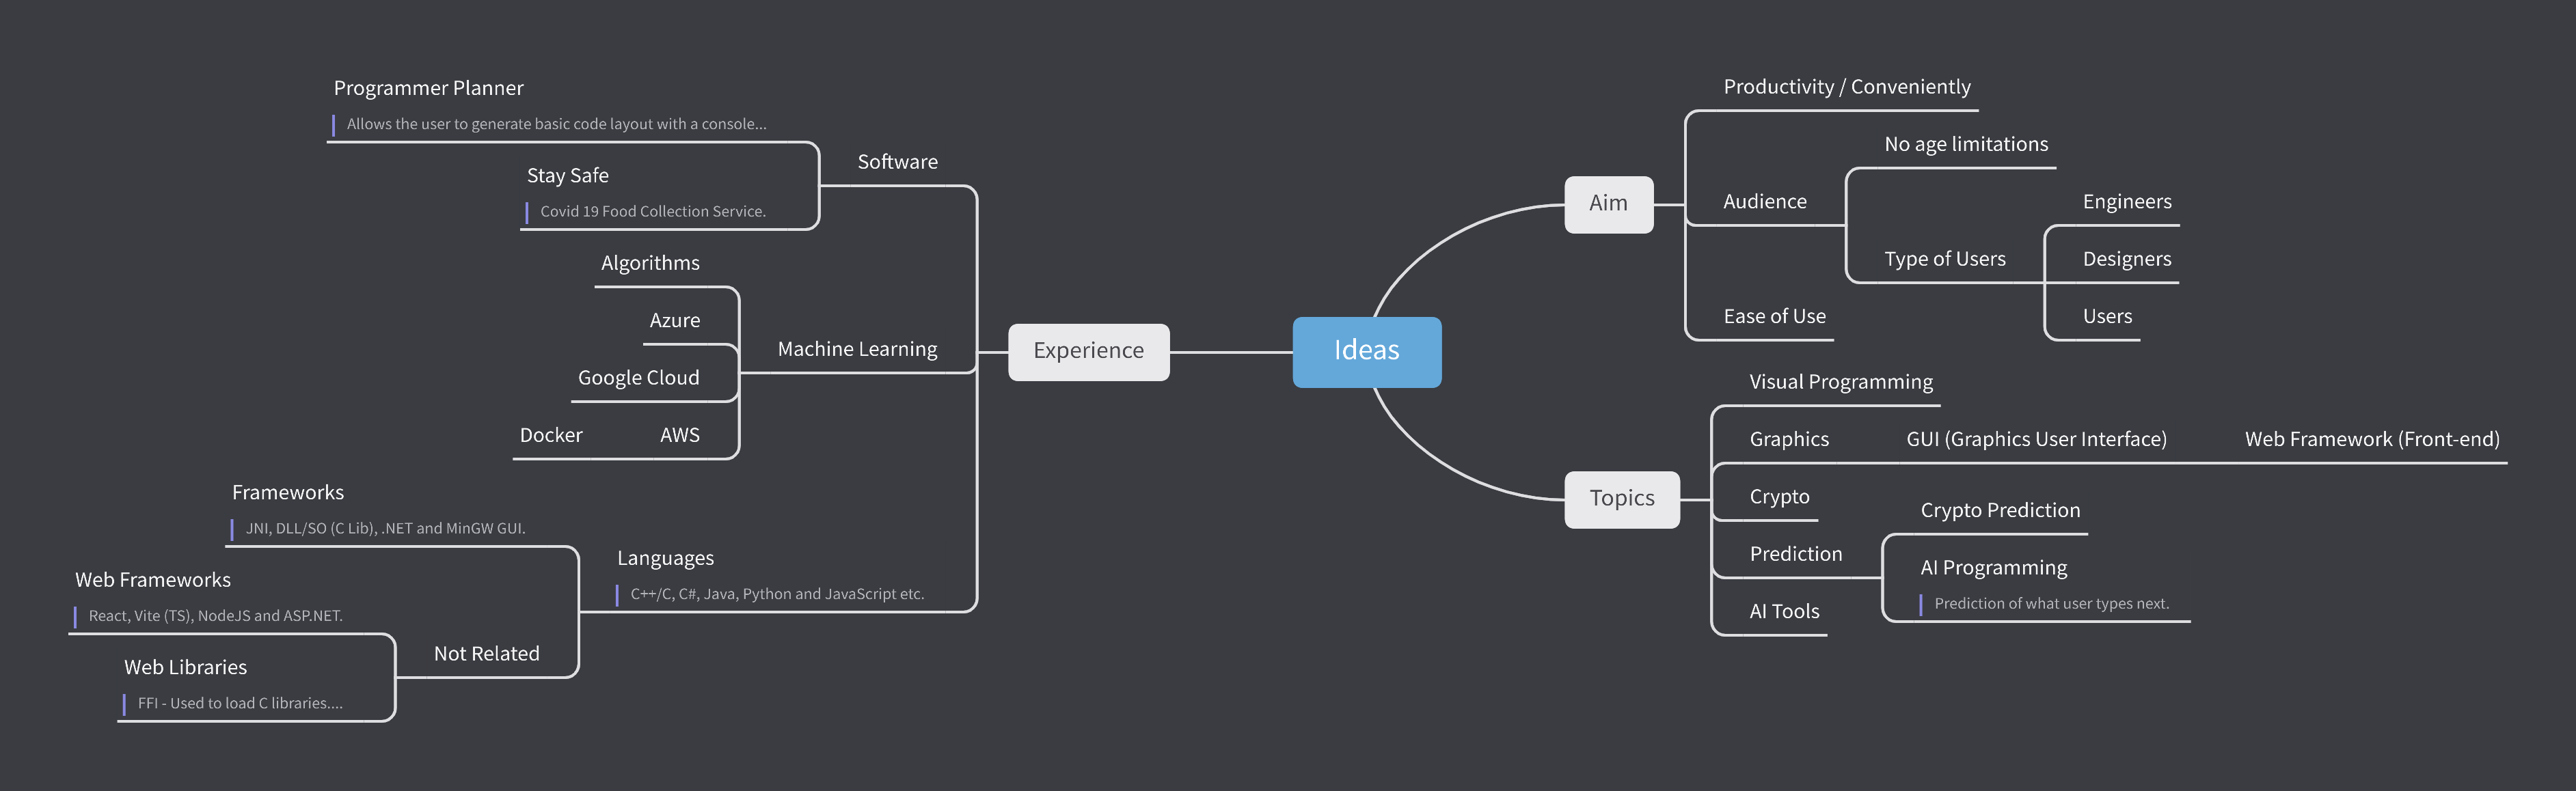
\includegraphics[height=.83\textheight, width=1.30\textwidth]{Figures/mindmap-ideas.png}
          \caption{VisualPro Ideas Mindmap}
        \end{figure}
      \end{landscape}
      %SUBSECTION END

      %SUBSECTION LANDSCAPE
      \begin{landscape}
        \thispagestyle{fancylandscape}
        \subsection{Mindmap - VisualPro}
        This mindmap displays existing and future libraries or problems within the final project that may prove resourceful within the development of VisualPro.
        \begin{figure}[h]
          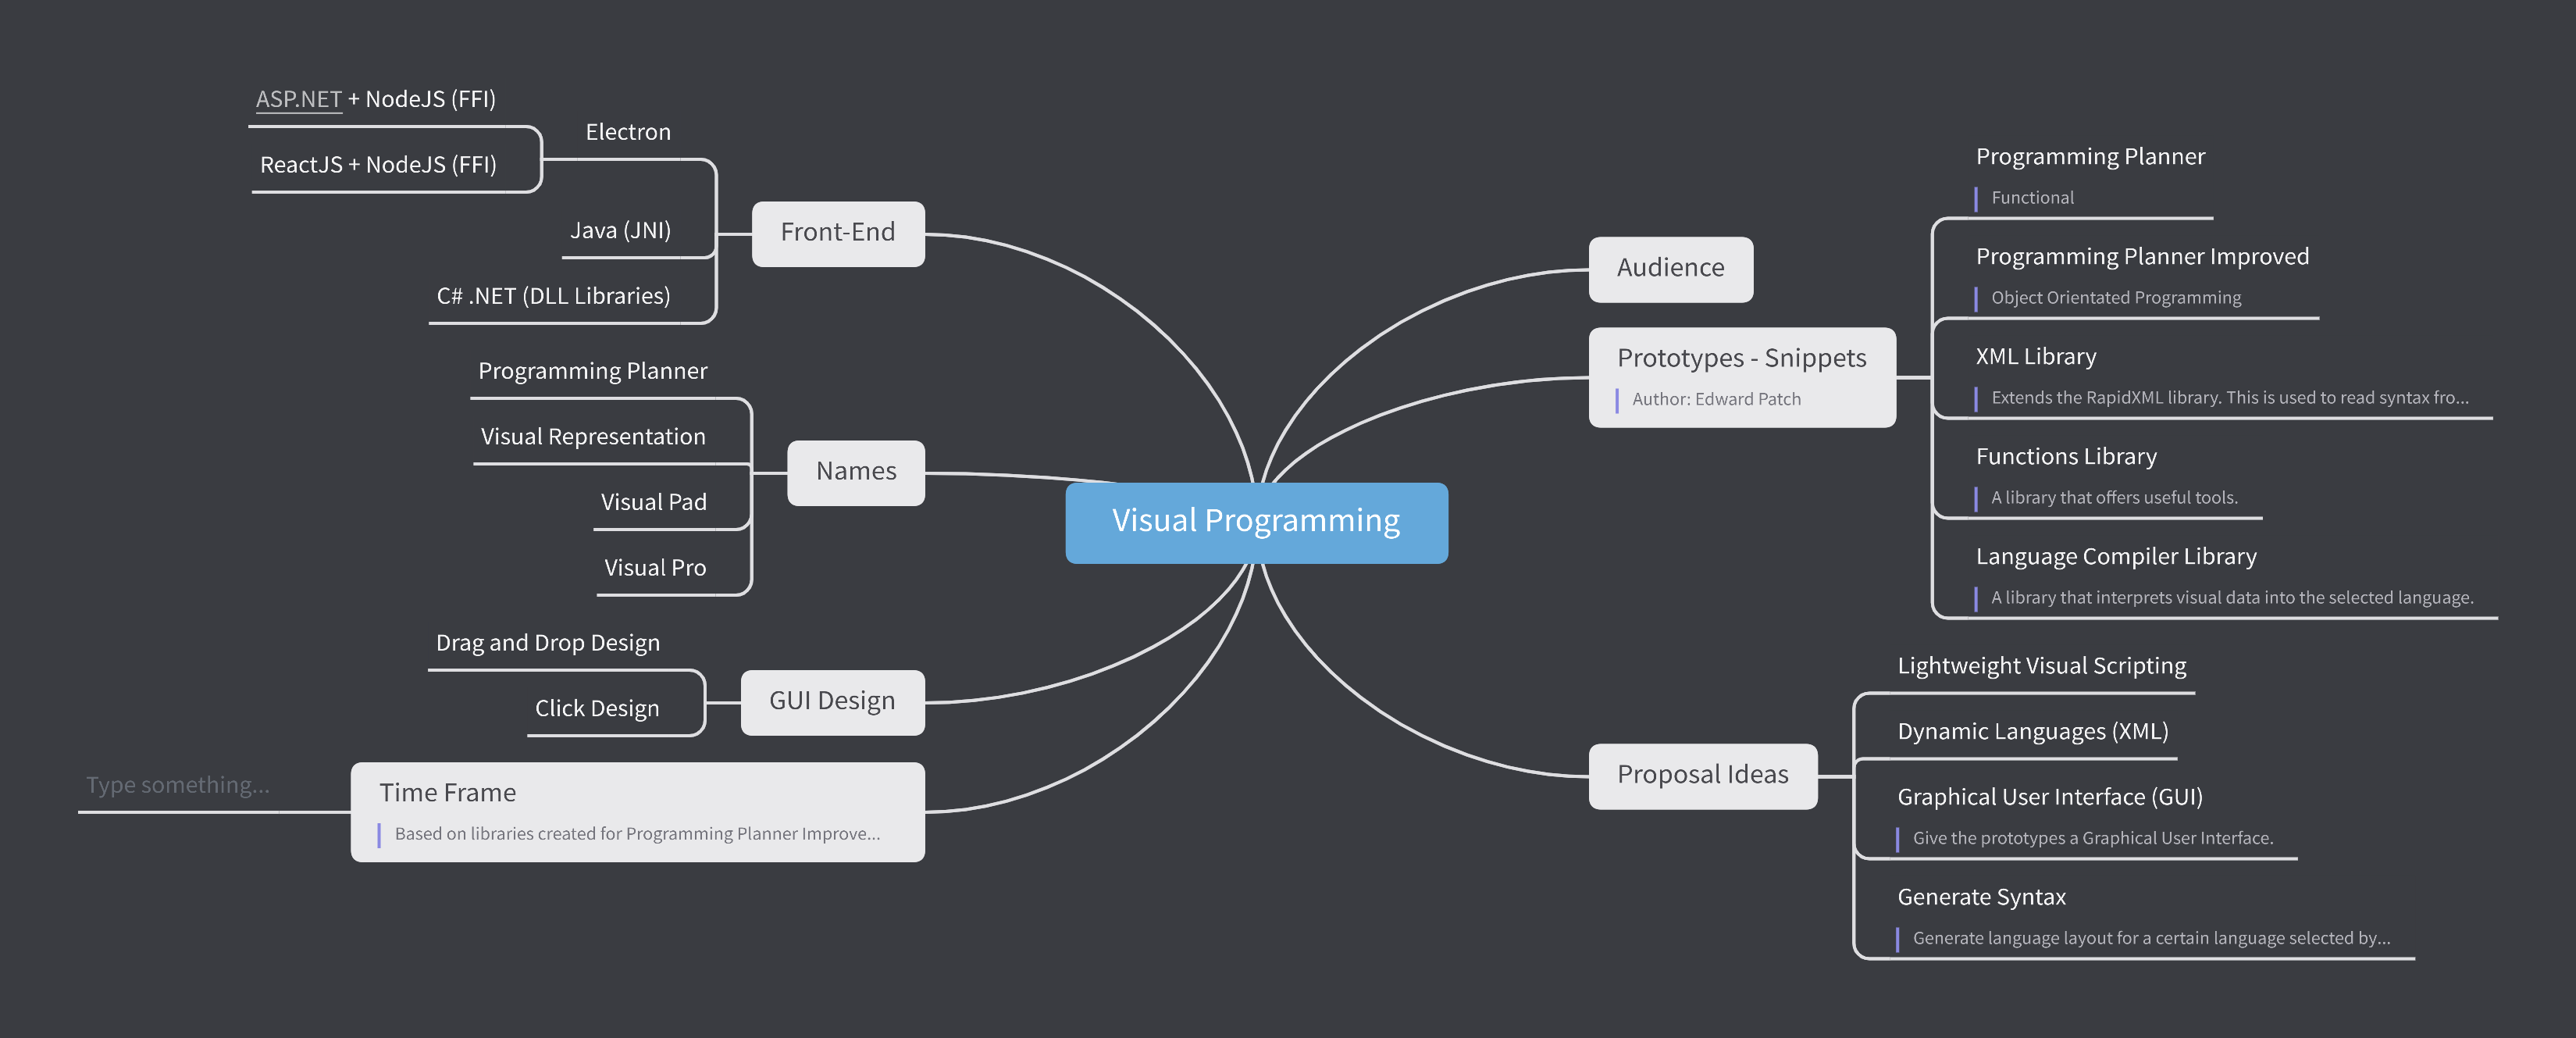
\includegraphics[height=.83\textheight, width=1.30\textwidth]{Figures/mindmap-vp.png}
          \caption{VisualPro Mindmap}
        \end{figure}
      \end{landscape}
      %SUBSECTION END

    \section{Terminology}
      List of terminologies used in this document:-
      \begin{itemize}
        \item Graphical User Interface (GUI).
        \item Extensible Markup Language (XML).
        \item Dynamic-Link Library (DLL).
      \end{itemize}

    \section{Conclusion}
    
	\nocite{*}
	\renewcommand\refname{\section{Reference List}}
	\small{\bibliographystyle{IEEEtran}
    \bibliography{ref}}
\end{document}